\documentclass[11pt]{article}
\usepackage{anysize} 
\marginsize{2cm}{2cm}{2cm}{2cm} 

\usepackage{multirow}
\usepackage{tabularx}
\usepackage{longtable}
\usepackage[utf8]{inputenc}
\usepackage[spanish]{babel}
\usepackage{hyperref}
\usepackage{fixltx2e}
\usepackage{mathtools}
\usepackage{amsmath}
\usepackage{graphicx}
\usepackage{adjustbox}
\usepackage{subcaption}

%%%%%%%%%%%%%%%%%%%%%%%%%%%%%%%%%%%%%%%%%%%%%%%%%
%	headers & footers							%
%%%%%%%%%%%%%%%%%%%%%%%%%%%%%%%%%%%%%%%%%%%%%%%%%
\usepackage{fancyhdr}
\pagestyle{fancy}
\fancyhf{}
\rhead{Taller de Sistemas Computacionales}
\lhead{Segundo Semestre 2014}
\rfoot{Página \thepage}

%%%%%%%%%%%%%%%%%%%%%%%%%%%%%%%%%%%%%%%%%%%%%%%%%
%	comandos									%
%%%%%%%%%%%%%%%%%%%%%%%%%%%%%%%%%%%%%%%%%%%%%%%%%

\newcommand{\labno}{1}
\newcommand{\labtitle}{Taller de Sistemas Computacionales}
\newcommand{\nameone}{Iván González López}
\newcommand{\emailone}{ivan.gonzalezlo@alumnos.usm.cl}
\newcommand{\rolone}{2973523-9}
\newcommand{\nametwo}{Guillermo Baeza}
\newcommand{\emailtwo}{guillermo.baeza@alumnos.usm.cl}
\newcommand{\roltwo}{2973600-6}

\begin{document}
\begin{titlepage}
\begin{center}

%%%%%%%%%%%%%%%%%%%%%%%%%%%%%%%%%%%%%%%%%%%%%%%%%
%	título página inicial						%
%%%%%%%%%%%%%%%%%%%%%%%%%%%%%%%%%%%%%%%%%%%%%%%%%


\includegraphics[width=70pt]{logos/utfsm.pdf} \\
{\Large \textsc{Universidad Técnica Federico Santa María} \\}
{\Large \textsc{Departamento de Informática} \\ \vspace{4pt}}
{\rule[13pt]{\textwidth}{1pt} \\ \vspace{25pt}}
{\LARGE \textsc{Tarea No. \labno} \\}
{\LARGE \textsc{\labtitle} \\ \vspace{50pt}}

%%%%%%%%%%%%%%%%%%%%%%%%%%%%%%%%%%%%%%%%%%%%%%%%%
%	autores										%
%%%%%%%%%%%%%%%%%%%%%%%%%%%%%%%%%%%%%%%%%%%%%%%%%
\begin{minipage}{0.4\textwidth}
\begin{flushleft}
{\large \nameone} \\
\emailone \\
\rolone
\end{flushleft}
\end{minipage}
\hfill
\begin{minipage}{0.4\textwidth}
\begin{flushright}
{\large \nametwo} \\
\emailtwo \\
\roltwo
\end{flushright}
\end{minipage}
\end{center}
\end{titlepage}


\section{Descripción}
Mediante el software de virtualización VirtualBox, se crearán dos máquinas virtuales de la distribución de Linux CentOS 6.5 x86, en su versión desktop y minimal (sin entorno gráfico). Para ambas versiones, se registrará su tiempo de instalación, uso de recursos, y además de configurar una red NAT y otra bridge dentro de ellas.   

\section{Análisis y Desarrollo}
\subsection{Instalación}
Las imágenes iso, fueron descargadas del repositorio de la Universidad, \url{ftp://ftp.inf.utfsm.cl/pub/Linux/CentOS/6.5/isos/i386/}. Las máquinas virtuales, fueron configuradas para disponer de una memoria principal de 1024 MB y una memoria secundaria de almacenamiento de 10 GB.
	\subsubsection{CentOS minimal version}
		\begin{enumerate}
			\item 
				\begin{minipage}[t]{\linewidth}
			          \raggedright
			          \adjustbox{valign=t}{
			            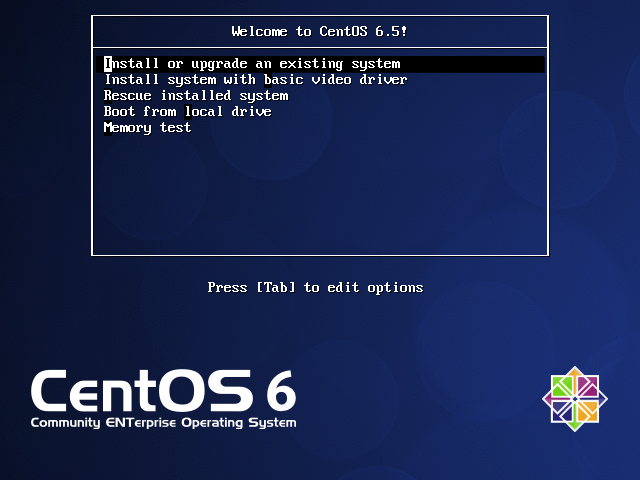
\includegraphics[width=.45\linewidth]{ss/MIN/instalacion/primera.png}
			          }
			          \medskip
			          \\Del menú de inicio, seleccionar la primera opción, instalar o actualizar un sistema existente.
			    \end{minipage}
			
			\item Puesto que se trata de un máquina virtual, omitir el chequeo de los dispositivos de DVD o usb.
			\item Elegir el idioma utilizado para realizar la instalación.
			\item Elegir la distribución del teclado.

			\item 
				\begin{minipage}[t]{\linewidth}
			          \raggedright
			          \adjustbox{valign=t}{
			            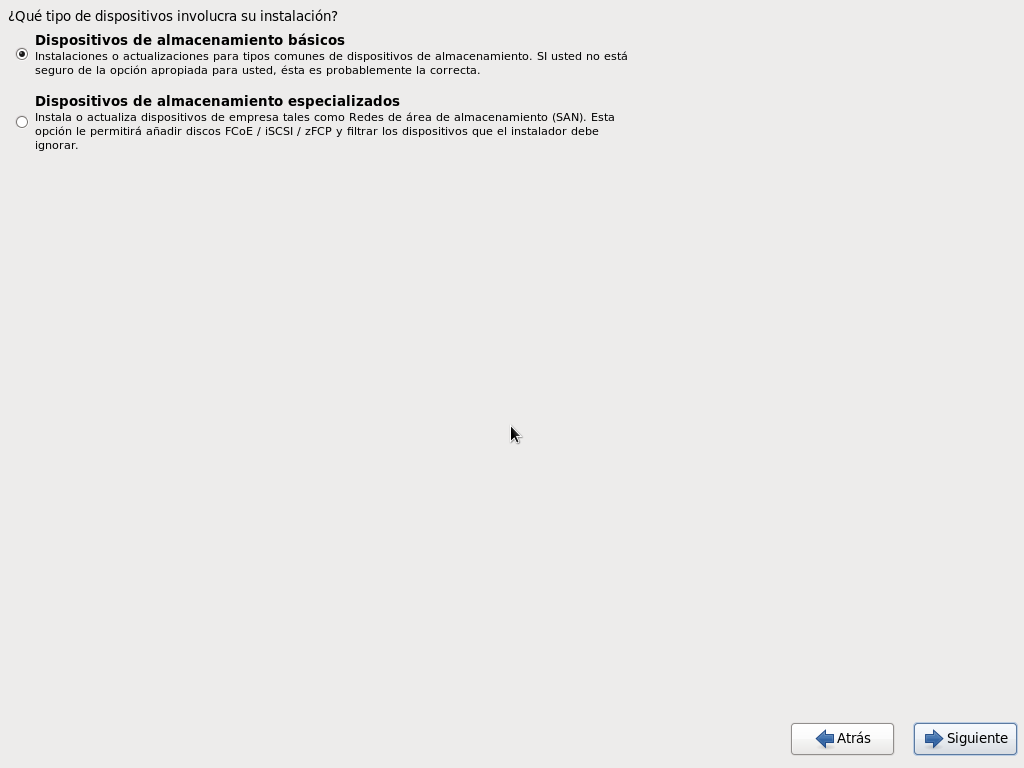
\includegraphics[width=.45\linewidth]{ss/MIN/instalacion/diskN.png}
			          }
			          \medskip
			          \\En caso de contar con dispositivos de almacenamiento especializados como iSCSI, SAN, etc, marcar la segunda opción, sino, la primera es la que se elige. Dar en siguiente.
			    \end{minipage}			

			\item El disco que se utilizará para la instalcion ha sido detectado, confirmar el descarte de todos los datos.
			\item Escribir el nombre del computador o hostname.
			\item 				
				\begin{minipage}[t]{\linewidth}
			          \raggedright
			          \adjustbox{valign=t}{
			            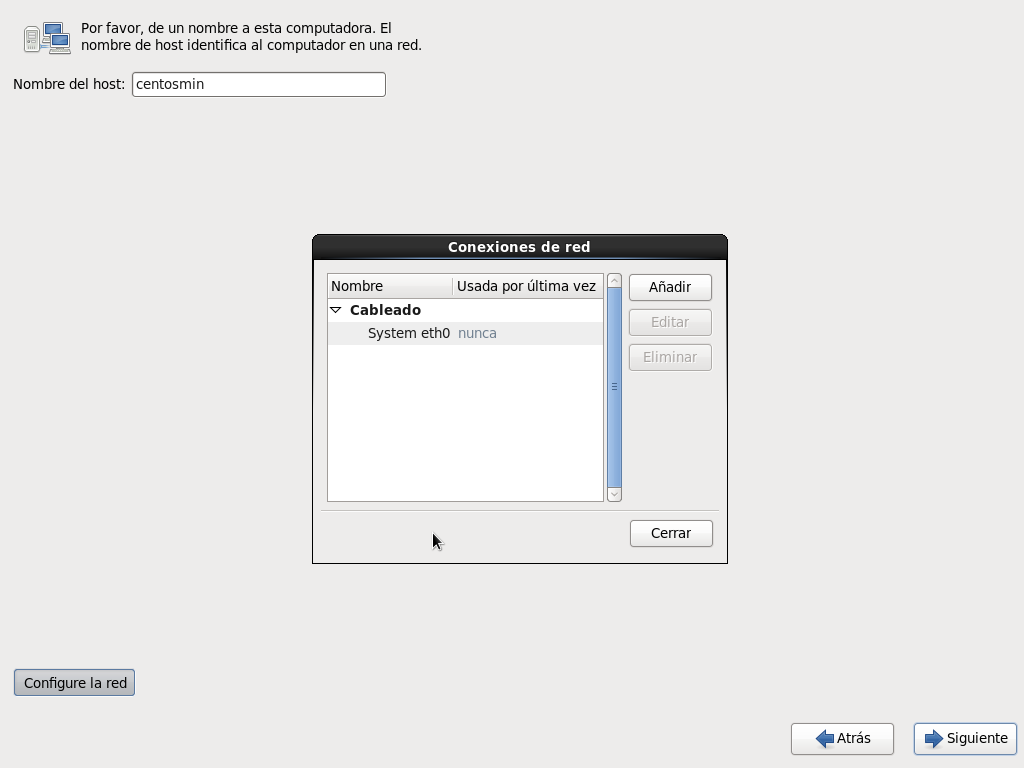
\includegraphics[width=.45\linewidth]{ss/MIN/instalacion/red.png}
			          }
			          \medskip
			          \\Dar click en el boton \textbf{Configure la red}. Seleccionar la interfas System eth0.
			    \end{minipage}	

			\item
				\begin{minipage}[t]{\linewidth}
			          \raggedright
			          \adjustbox{valign=t}{
			            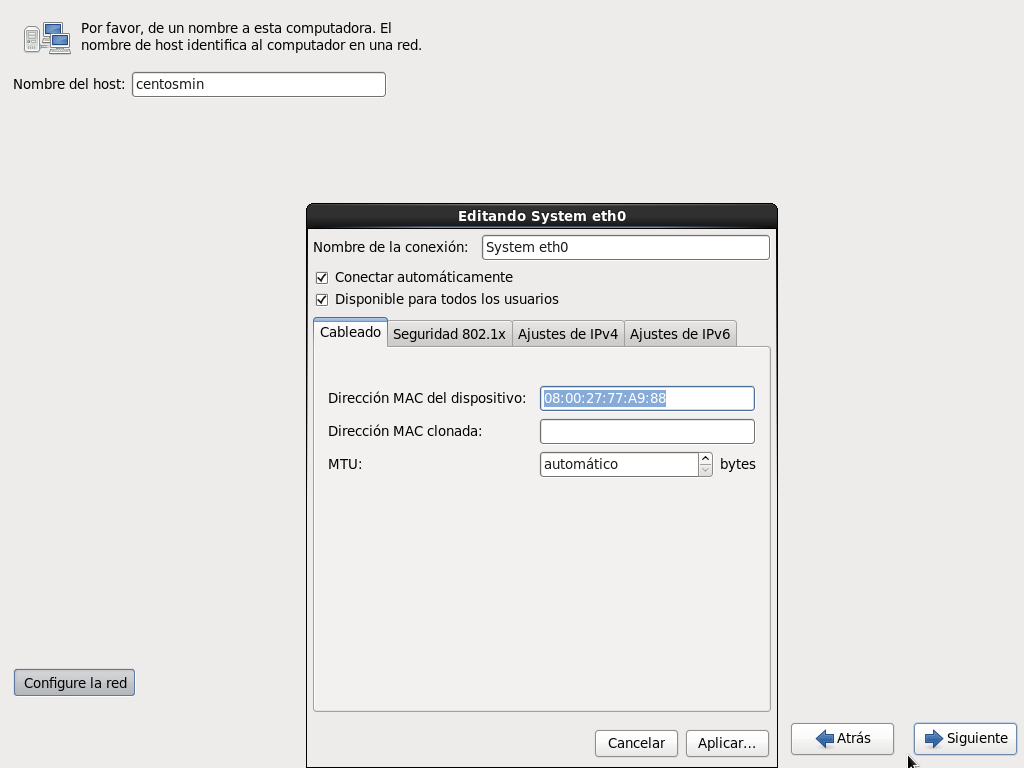
\includegraphics[width=.45\linewidth]{ss/MIN/instalacion/red2.png}
			          }
			          \medskip
			          \\Posteriormente, dar click en editar y marcar el checkbox \textbf{Conectar automáticamente}. Dar click a Aplicar. Luego hacer click en Cerrar y después Siguiente.
			    \end{minipage}	

			\item 
				\begin{minipage}[t]{\linewidth}
			          \raggedright
			          \adjustbox{valign=t}{
			            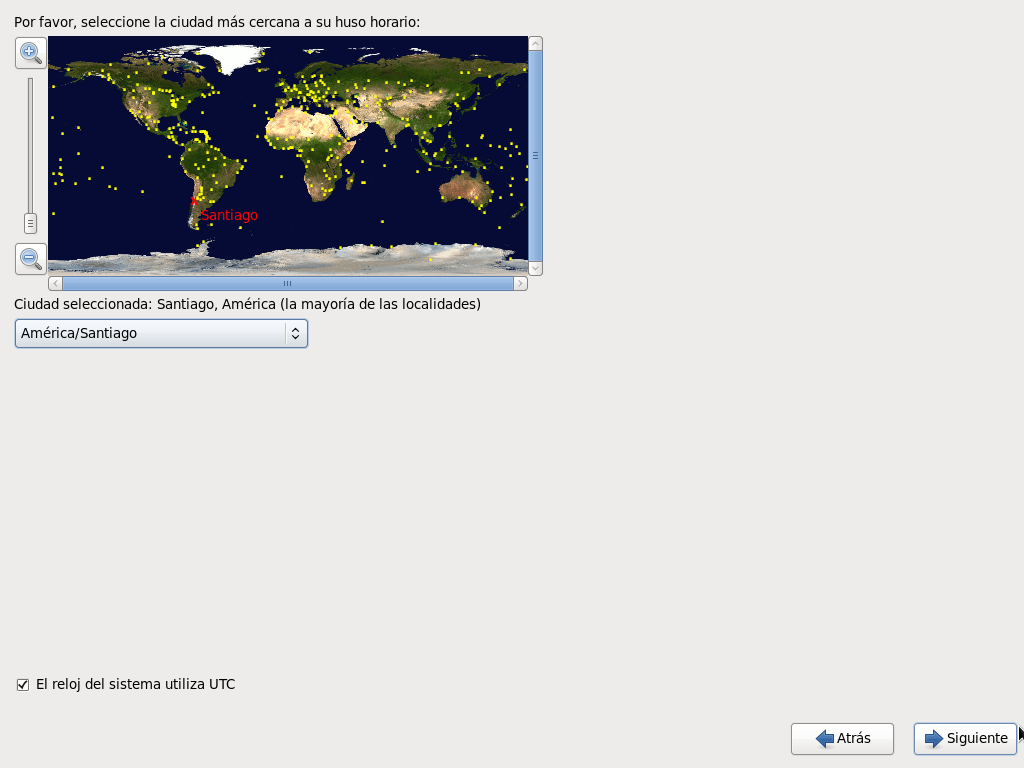
\includegraphics[width=.45\linewidth]{ss/MIN/instalacion/huso.png}
			          }
			          \medskip
			          \\Elegir la zona horaria, dependiendo de la ubicación geográfica. Siguiente. 
			    \end{minipage}	
			
			\item Escribir la contraseña del usuario root. Confirmar la contraseña. Siguiente.
			\item 
				\begin{minipage}[t]{\linewidth}
			          \raggedright
			          \adjustbox{valign=t}{
			            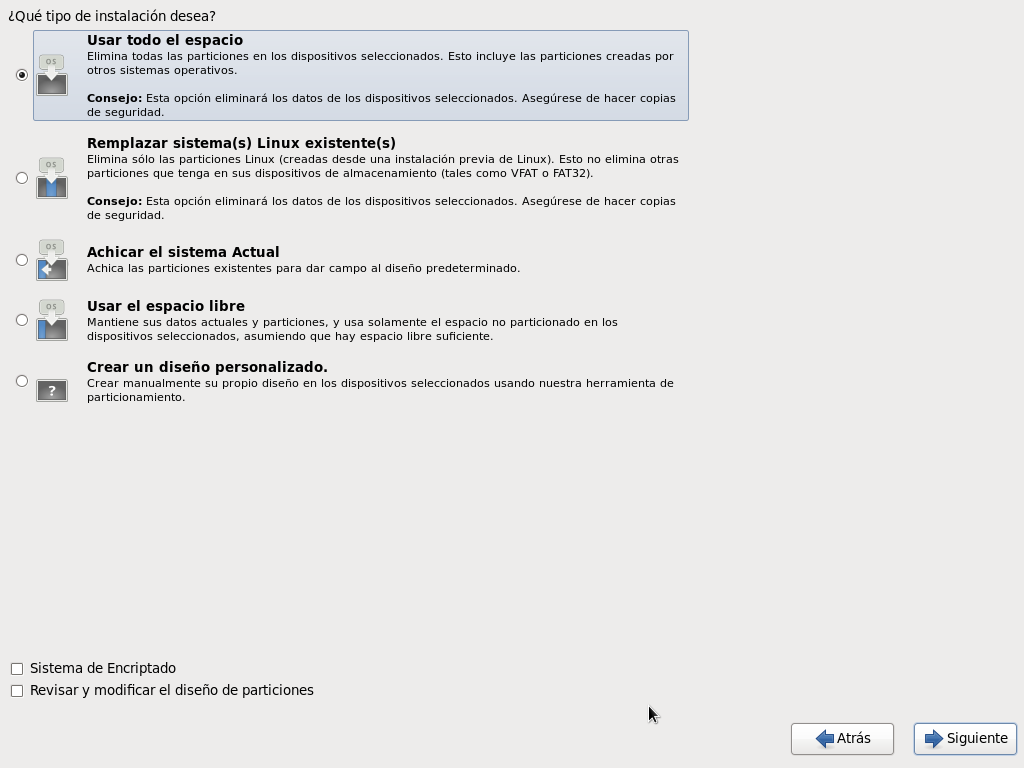
\includegraphics[width=.45\linewidth]{ss/MIN/instalacion/particion.png}
			          }
			          \medskip
			          \\Proceso de particionado del disco virtual. Elegir usar todo el espacio. Siguiente. 
			    \end{minipage}	

			\item Confirmar \textbf{Escribir cambios al disco}.

			\item 
				\begin{minipage}[t]{\linewidth}
			        \raggedright
			        \adjustbox{valign=t}{
			        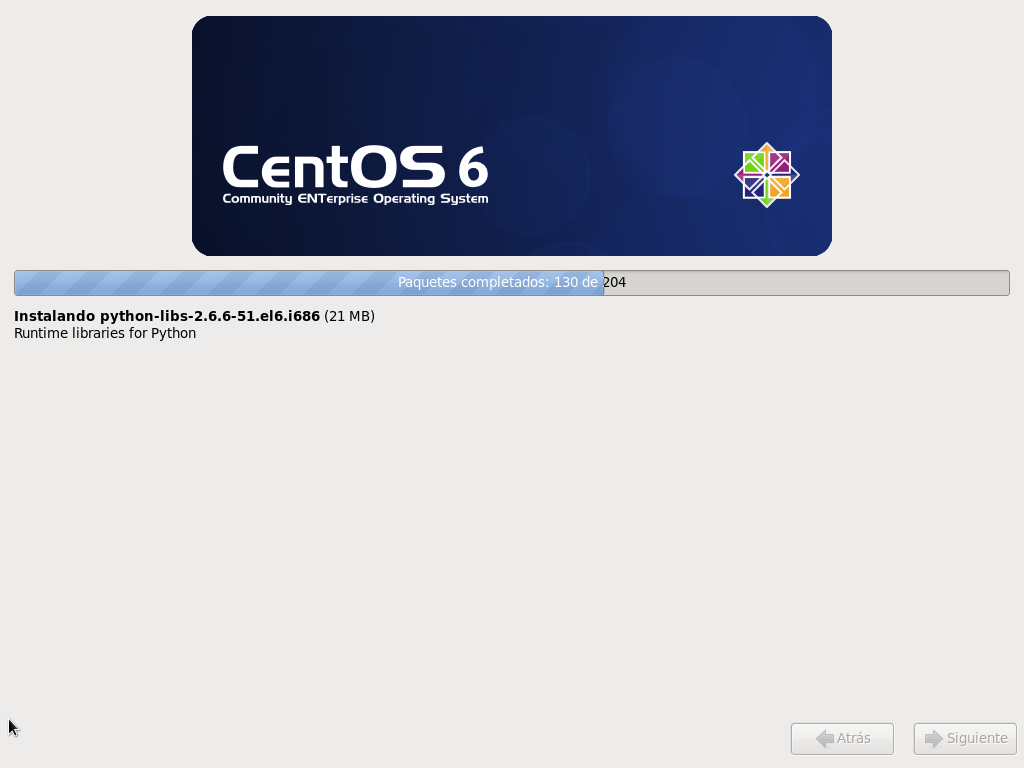
\includegraphics[width=.45\linewidth]{ss/MIN/instalacion/instalacion.png}
			        }
			        \medskip
			        \\Comienza el proceso de instalación. 
		        \end{minipage}	

		    \item 
		    	\begin{minipage}[t]{\linewidth}
			        \raggedright
			        \adjustbox{valign=t}{
			        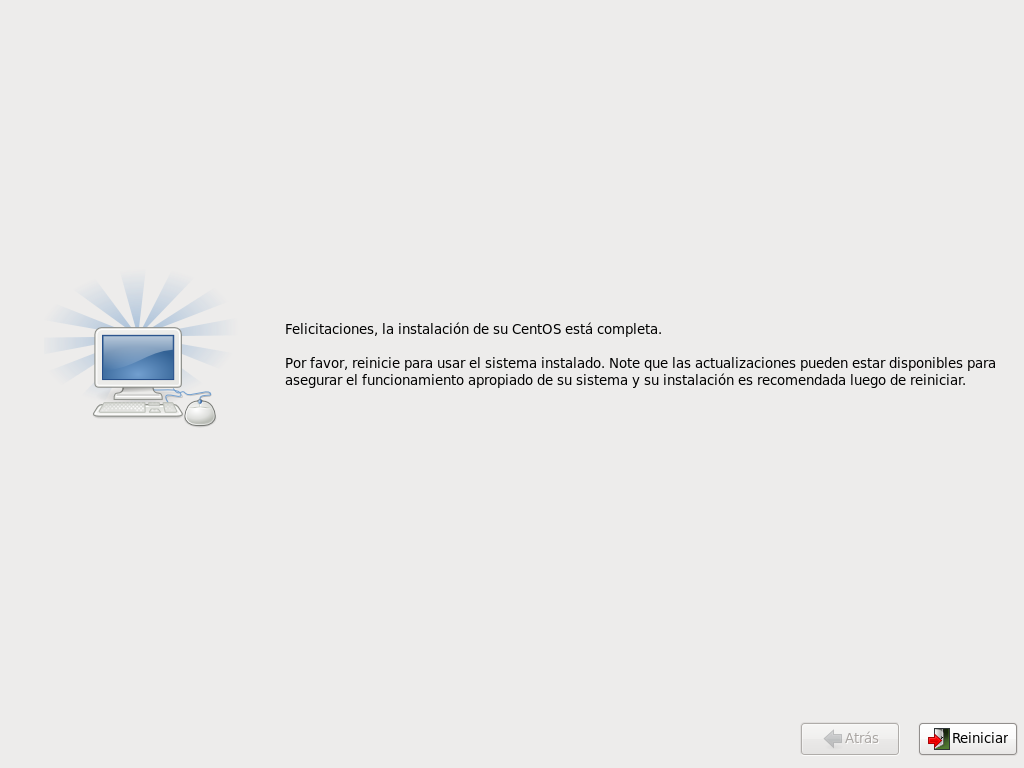
\includegraphics[width=.45\linewidth]{ss/MIN/instalacion/fin.png}
			        }
			        \medskip
			        \\Instalación finalizada. Reiniciar. 
		        \end{minipage}	

		   	\item 
		   		\begin{minipage}[t]{\linewidth}
			        \raggedright
			        \adjustbox{valign=t}{
			        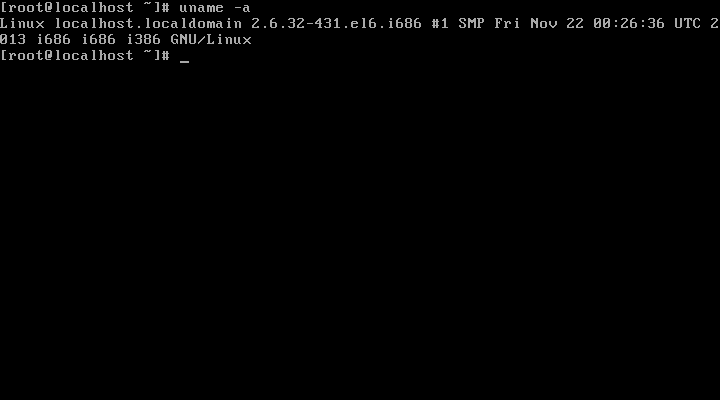
\includegraphics[width=.45\linewidth]{ss/MIN/instalacion/uname.png}
			        }
			        \medskip
			        \\Tipear el nombre de usuario root y su contraseña. Listo. 
		        \end{minipage}	

		    \item 
		    	\begin{minipage}[t]{\linewidth}
			        \raggedright
			        \adjustbox{valign=t}{
			        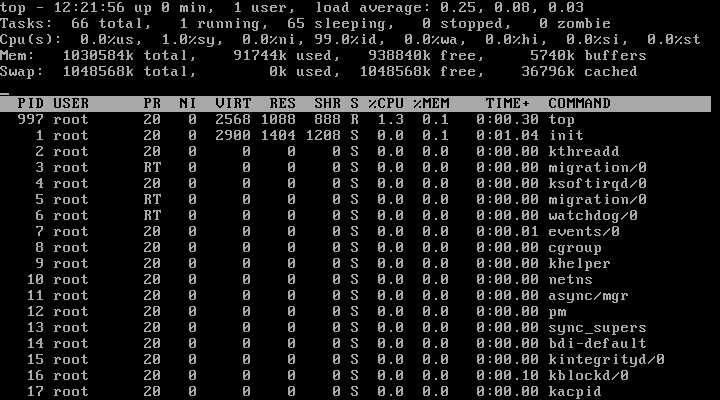
\includegraphics[width=.45\linewidth]{ss/MIN/instalacion/top.png}
			        }
			        \medskip
			        \\Comando top, para visualizar la utilización de recursos del sistema. 
		        \end{minipage}
		\end{enumerate}

	\subsubsection{CentOS desktop version}	
		\begin{enumerate}
			\item 
				\begin{minipage}[t]{\linewidth}
			        \raggedright
			        \adjustbox{valign=t}{
			        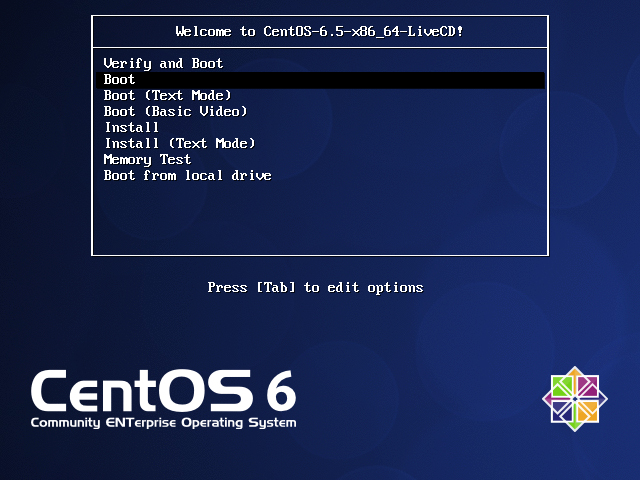
\includegraphics[width=.45\linewidth]{ss/FULL/instalacion/boot-menu.png}
			        }
			        \medskip
			        \\Del menú de inicio, seleccionar la opción \textbf{Boot} o iniciar. 
		        \end{minipage}

		    \item
		    	\begin{minipage}[t]{\linewidth}
			        \raggedright
			        \adjustbox{valign=t}{
			        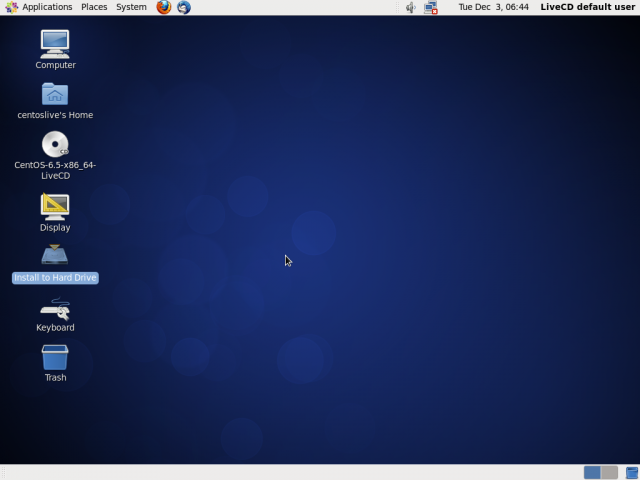
\includegraphics[width=.45\linewidth]{ss/FULL/instalacion/desktop.png}
			        }
			        \medskip
			        \\Dentro del escritorio, hacer doble click sobre el ícono \textbf{Install to Hard Drive}. 
		        \end{minipage}	

		    \item Hacer click en Siguiente, en el asistente de instalación.
		    \item Seleccionar la distribución del teclado. Siguiete.
		    \item 
		    	\begin{minipage}[t]{\linewidth}
			        \raggedright
			        \adjustbox{valign=t}{
			        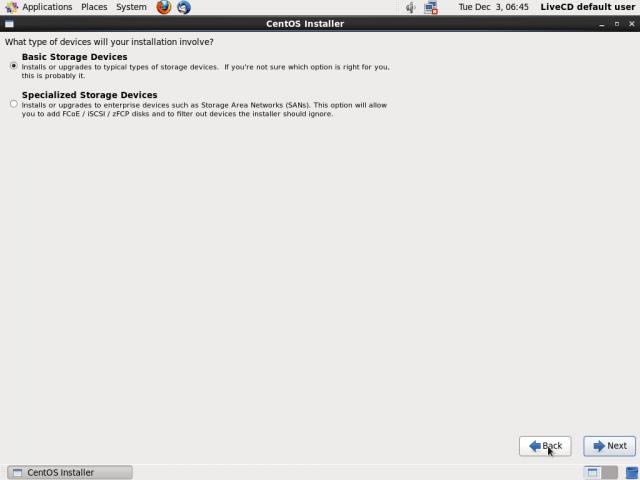
\includegraphics[width=.45\linewidth]{ss/FULL/instalacion/almacenamiento.png}
			        }
			        \medskip
			        \\En caso de contar con dispositivos de almacenamiento especializados como iSCSI, SAN, etc, marcar la segunda opción, sino, la primera es la que se elige. Dar en siguiente. 
		        \end{minipage}	

		    \item Escribir el nombre del computador o hostname.
		    \item Escoger la zona horaria, dependiendo de la ubicación geográfica. Siguiente.
		    \item 
		    	\begin{minipage}[t]{\linewidth}
			        \raggedright
			        \adjustbox{valign=t}{
			        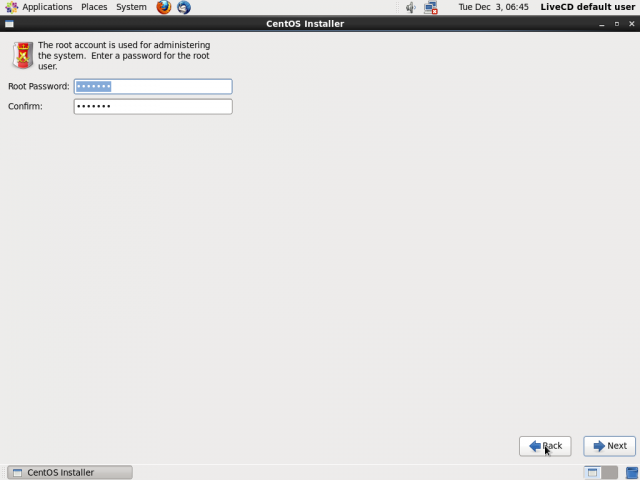
\includegraphics[width=.45\linewidth]{ss/FULL/instalacion/root-password.png}
			        }
			        \medskip
			        \\Suministrar la contraseña del usuario root. Confirmar. Siguiente. 
		        \end{minipage}

		    \item 
		    	\begin{minipage}[t]{\linewidth}
			        \raggedright
			        \adjustbox{valign=t}{
			        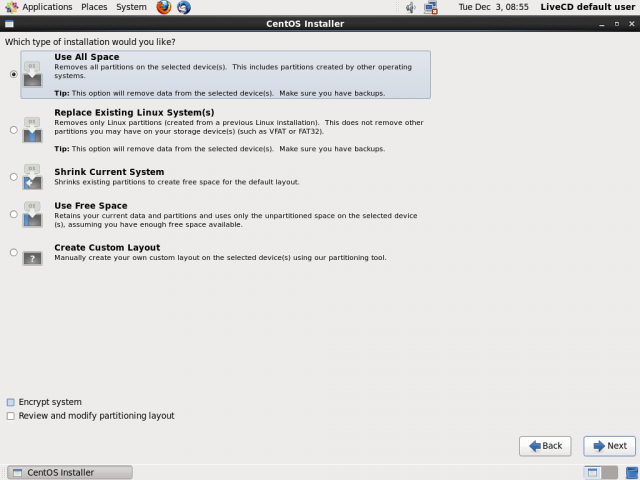
\includegraphics[width=.45\linewidth]{ss/FULL/instalacion/particion.png}
			        }
			        \medskip
			        \\Proceso de particionado del disco virtual. Elegir usar todo el espacio. Siguiente. 
		        \end{minipage}

		    \item 
		    	\begin{minipage}[t]{\linewidth}
			        \raggedright
			        \adjustbox{valign=t}{
			        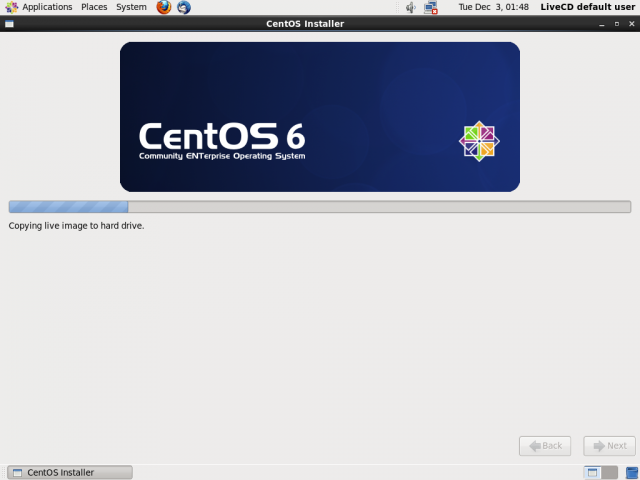
\includegraphics[width=.45\linewidth]{ss/FULL/instalacion/instalacion.png}
			        }
			        \medskip
			        \\Instalación del sistema Se copian todos los archivos necesarios al disco virtual. 
		        \end{minipage}

		    \item
		    	\begin{minipage}[t]{\linewidth}
			        \raggedright
			        \adjustbox{valign=t}{
			        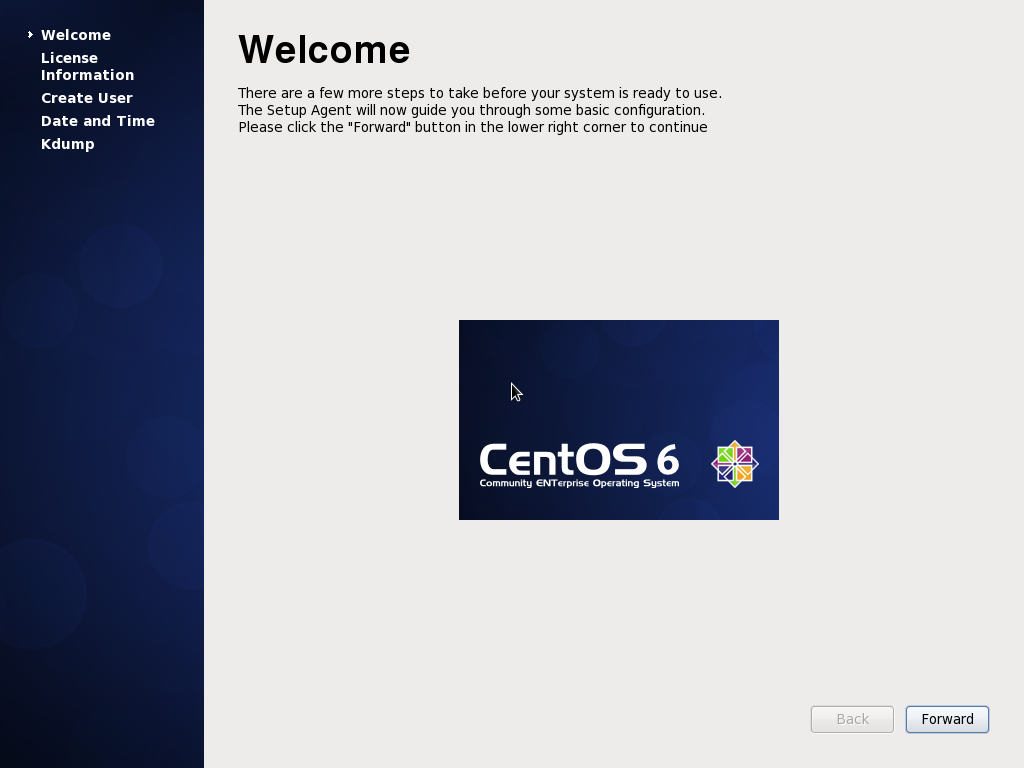
\includegraphics[width=.45\linewidth]{ss/FULL/instalacion/setup.png}
			        }
			        \medskip
			        \\Proceso de configuración post instalación. Siguiente. 
		        \end{minipage}

		    \item 
		    	\begin{minipage}[t]{\linewidth}
			        \raggedright
			        \adjustbox{valign=t}{
			        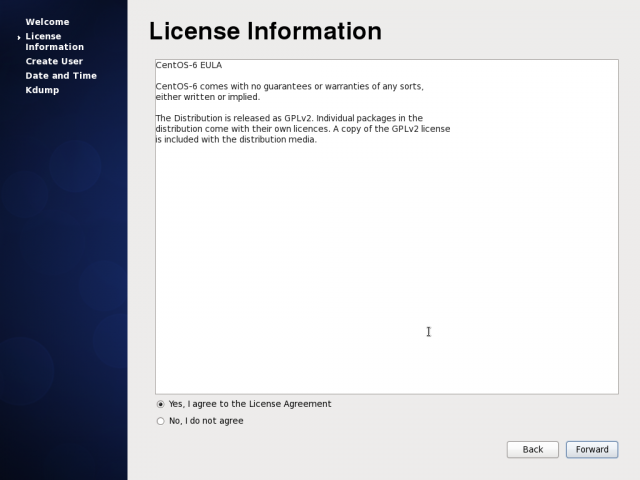
\includegraphics[width=.45\linewidth]{ss/FULL/instalacion/licencia.png}
			        }
			        \medskip
			        \\Leer y aceptar acuerdo de licencia. Siguiente. 
		        \end{minipage}

		    \item Crear una nueva cuenta de usuario, para poder utilizar el sistema.
		    \item Ingresar hora y fechas actuales.
		    \item Kdump. Este es el último del asistente de configuración, donde pregunta si Kdump debe ser activado o no. Dejar los valores por defecto. Finalizar.

		    \item
		    	\begin{minipage}[t]{\linewidth}
			        \raggedright
			        \adjustbox{valign=t}{
			        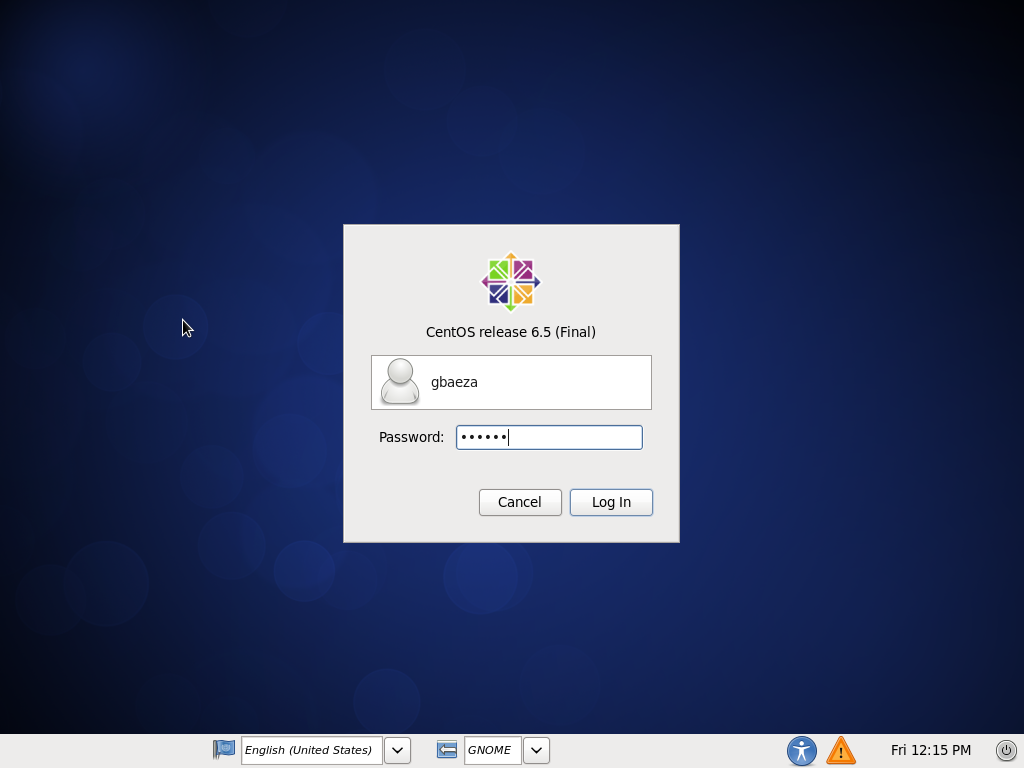
\includegraphics[width=.45\linewidth]{ss/FULL/instalacion/login.png}
			        }
			        \medskip
			        \\Después de reiniciado el sistema, se presentará la pantalla de login para iniciar sesión. 
		        \end{minipage}

	        \item
	        	\begin{minipage}[t]{\linewidth}
			        \raggedright
			        \adjustbox{valign=t}{
			        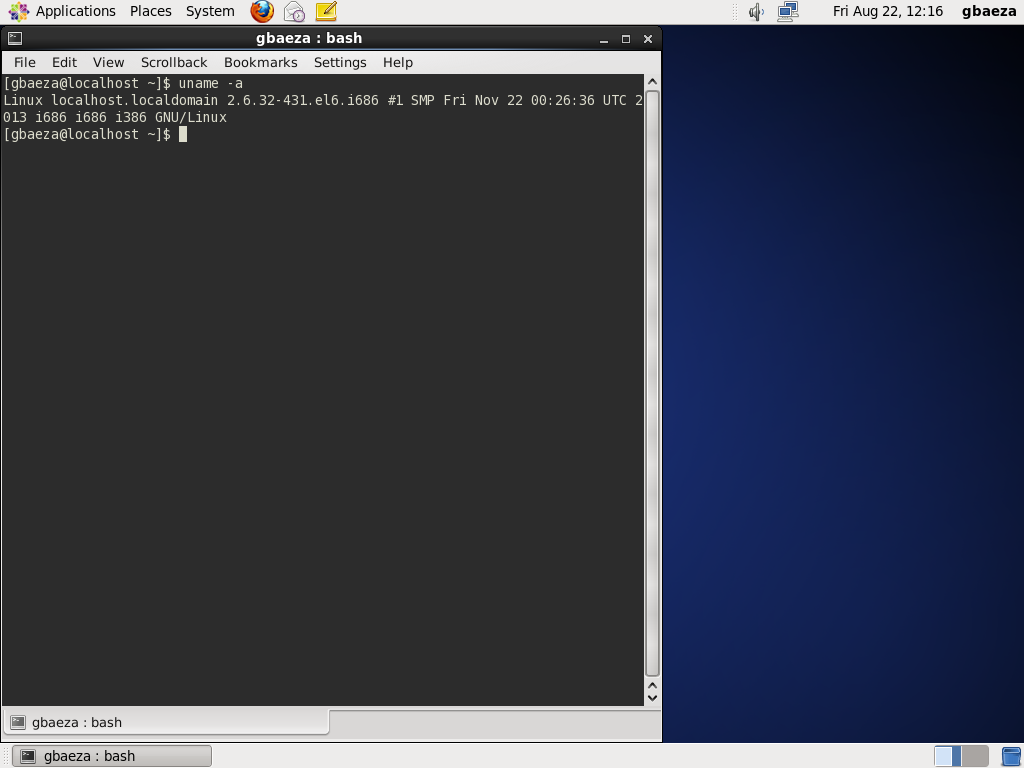
\includegraphics[width=.45\linewidth]{ss/FULL/instalacion/CentOS.png}
			        }
			        \medskip
			        \\Después de iniciar sesión, se presentará el escritorio de CentOS 6.5 Desktop.
		        \end{minipage}

		    \item
	        	\begin{minipage}[t]{\linewidth}
			        \raggedright
			        \adjustbox{valign=t}{
			        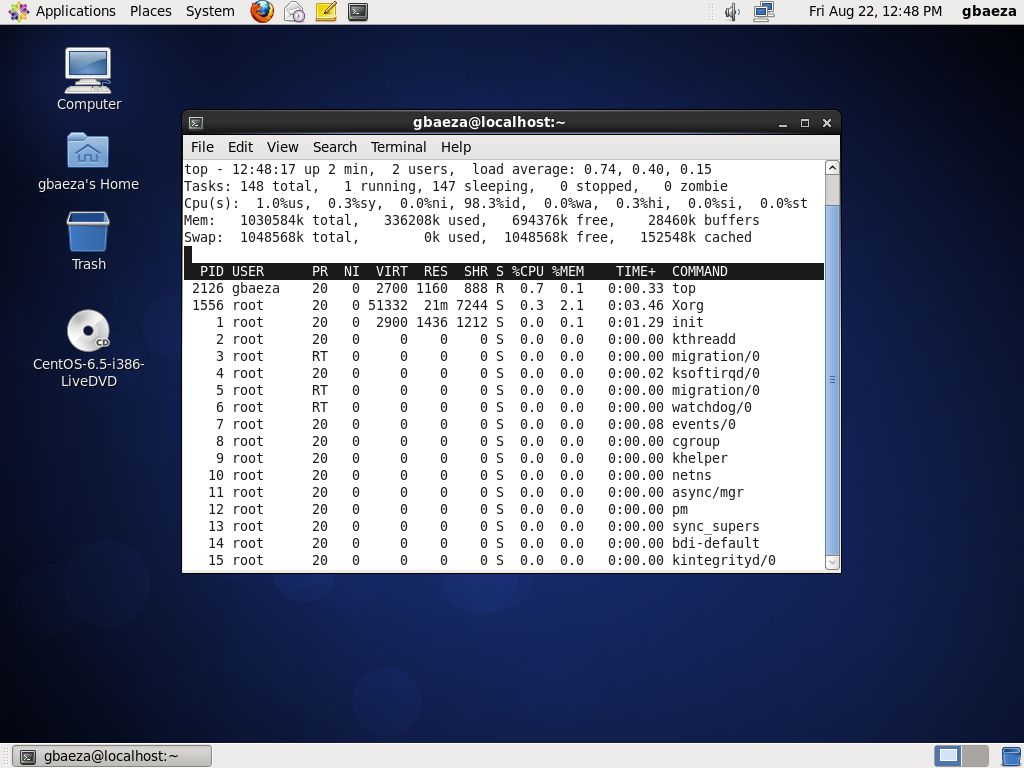
\includegraphics[width=.45\linewidth]{ss/FULL/instalacion/top.png}
			        }
			        \medskip
			        \\Comando top, para visualizar la utilización de recursos del sistema.
		        \end{minipage}
		    \end{enumerate}

		    Respecto del consumo de recursos de ambos sistemas, se podía anticipar con certeza que, CentOS en su versión mínima, es más eficiente que en su versión de escritorio, dado que, entre otras diferencias, la versión mínima no cuenta con un entorno de escritorio gráfico como Gnome. Es así como CentOS mínimo, ocupa alrededor de $91.744 [MB]$ de memoria principal; en cambio CentOS desktop ocupa alrededor de $336.208 [MB]$ de memoria principal.
\subsection{Configuración de Red}
\subsubsection{Red NAT}
	En VirtualBox, este es el modo de red por defecto en las nuevas máquinas virtuales. Cuando el sistema operativo invitado inicia, típicamente utiliza DHCP para obtener una dirección IP. VirtualBox alineará esta petición DHCP y le comunicará al SO invitado su dirección IP asignada y la puerta de enlace para el enrutamiento de las conecciones salientes. En este modo, cada máquina virtual es asignada a la misma dirección IP (10.0.2.15) porque cada una de estas piensa que están en su propia red aislada. Y cuando estas envían su tráfico a través de la puerta de enlace (10.0.2.2), VirtualBox reescribe los paquetes para hacerlos parecer que fueron enviados desde el Host, en vez del SO invitado (dentro del Host o huésped).
	Esto significa que el SO invitado, funcionará incluso si el Host se mueve desde una red a otra (como un notebook moviéndose en distintas ubicaciones), y desde conexiones inalámbricas a conexiones cableadas también. Lógicamente, una red de este tipo de ve de esta forma:

	\begin{figure}[ht]
	\center
	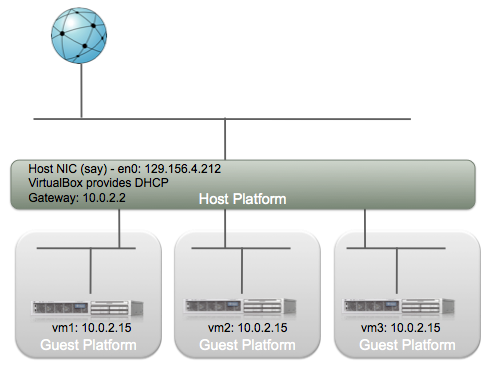
\includegraphics[width=0.5\linewidth]{ss/nat-network.png} 
	\caption{Esquema de una red NAT}
	\end{figure}


\subsubsection{Red bridge}
	Redes tipo bridge son usadas cuando se quiere que la máquina virtual sea un miembro completo de la red, i.e. que se comporte igual que la máquina huésped en la red.

	En este modo, un NIC virtual es ``puenteado'' a un NIC físico en el host, de la siguiente forma:

	\begin{figure}[ht]
	\center
	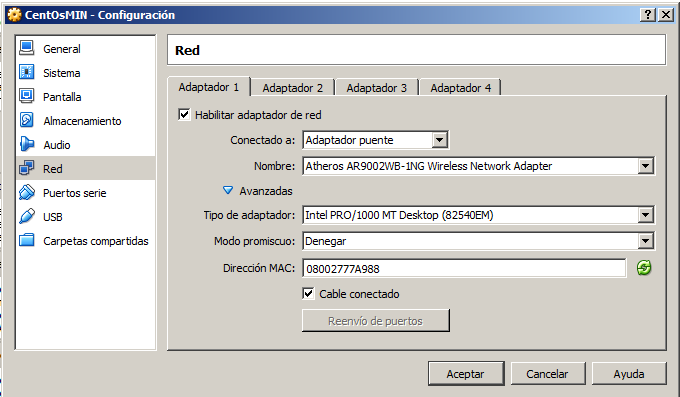
\includegraphics[width=0.5\linewidth]{ss/MIN/bridge/bridge-mv-min.png}
	\end{figure}

	El efecto en esto es que cada MV tiene acceso a la red física en la misma forma que el host. Puede acceder cualquier servicio en la red como por ejemplo servicios DHCP externos, servicios de búsqueda de nombre e información de ruteo, tal como el host lo hace. Lógicamente la red se ve de esta forma:

	\begin{figure}[ht]
	\center
	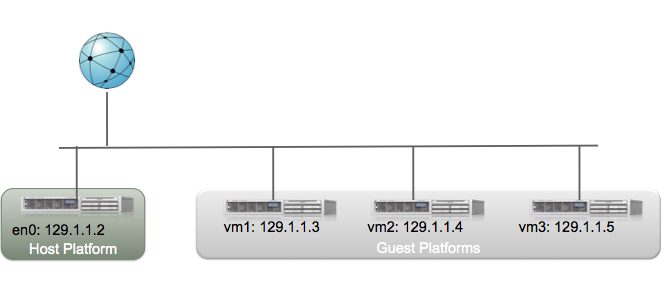
\includegraphics[width=0.75\linewidth]{ss/bridge-network.png} 
	\caption{Esquema de una red bridge} 
	\end{figure}


\section{Referencias}
	\begin{itemize}
		\item \url{https://blogs.oracle.com/fatbloke/entry/networking_in_virtualbox1}
		\item \url{http://serverfault.com/questions/229860/vmware-networking-mode-nat-or-bridged}
		\item \url{http://blog-rat.blogspot.com/2009/05/bridged-vs-host-only-vs-nat.html}
		\item \url{http://www.faqs.org/docs/securing/chap9sec90.html}
		\item \scriptsize \url{https://access.redhat.com/documentation/en-US/Red_Hat_Enterprise_Linux/4/html/Reference_Guide/ch-networkscripts.html}
		\item \scriptsize \url{http://extr3metech.wordpress.com/2013/05/23/configuring-network-in-centos-6-3-virtual-box-screenshots/}
	\end{itemize}
\end{document}
